\documentclass{article}
\usepackage[utf8]{inputenc}
%\usepackage{algorithm2e}
%\usepackage[linesnumbered]{algorithm2e}
%\usepackage[linesnumbered,ruled]{algorithm2e}
\usepackage[linesnumbered,ruled,vlined]{algorithm2e}
\usepackage{graphicx}

\graphicspath{ {./images/} }

\title{ Introducing realistic trading dynamics to the Bristol Stock Exchange}
\author{Dhammatorn Riewcharoon (dr17549) supervised by Dr.John Cartildge }
\date{February 2020}


\begin{document}
\tableofcontents{}
\maketitle

\section{Introduction}
\subsection{Contemporary Financial Market} 
The motivation of this project comes from the desire to understand and explore realism in simulating a contemporary financial stock market. When the first stock market was established, it was heavily reliant on human traders to offer a bid (buy order) and an ask( a sell order) at specific price in order to create a market. However, the contemporary financial market has become heavily reliant on automated trading systems for transactions, which raises the question of how these so-called trading systems can dominate the market than the other. Because a change in price can happen in less than a second with 6.43 billion trades happening each day, it is nearly impossible for any human to keep up.\cite{dailytrade} This change is inevitable and is now a common knowledge that no matter what we do, these trading systems will outperform human traders. It is commonly known in the U.S. that 80\% of the daily volume traded is executed by the automated systems \cite{percentAgent}. There is no doubt this number will increase in the following years due to the fact that robot trader or ``autonomous agents” requires less resources to perform the same or even better than human traders. 

Over the last two decades, there has been a significant increase and interest in study of the so called autonomous agents. With previous research from world renowned economist Vernon Smith who, in 1962, was able to prove that markets with limited unskilled participants was able to converge an equilibrium point, experimental economics became relevant \cite{smith1962}. Through Smith’s style experiment, researchers were able to experiment on autonomous agents which includes ZI-C, ZI-P, AA, Shaver, Klapan’s Sniper and many more. As these agents emerged, there has been an on-going study on their impact in a simulated market similar to Smith's experiments.  

By studying the behaviour of these agents, we now have a better insight on the impact of the agents in a market, more specifically in a simulated market where certain variables can be controlled. As a result, the These results which suggest AA doesn’t dominate often come from the fact that the adaptive agents, such as AA and ZI-P which response to the change in the market, does not do well in a market which reinforces realism. For example, a paper by Hanifan and Cartildge (2019) illustrated that  AA and ZI-P does not dominate in a market where reaction time (communication latency and trading latency) is taken into account \cite{foolsrush}. This paper will focus on an alternative method to introduce realism by using McG (shorthand for trading agents and model described in McGroarty et al.'s paper) agents to the BSE which similar experiments on existing agents will be performed \cite{McGroarty}. 

\section{Background}
\subsection{Limit Order Book}
The majority of large financial market now employs a Limit Order Book system, which can handle fast and effective trades in a matter of milliseconds. In a Limit Order Book system, a trader can submit either a buy (bid) or a sell (ask) with a price and a quantity. The Limit Order Book algorithm will then attempt to match a bid with another ask submitted with the price given. If there is no order on the other side of the book, the order will then sit on the list until it can be matched. 

In the BSE(Bristol Stock Exchange), the Limit Order Book system will, first match the ask order with the first bid order in a sorted list with the most price, then go down the list until all the quantity of the given ask order is complete. If there is not enough bid orders, the ask order will be posted back to the Limit Order ask side of the Book and vice versa for processing a bid order.

\subsubsection{Limit Price}
In a Limit Order Book market, a bid order must be submitted at the Bid limit price or lower while an ask order must be submitted at the Ask limit price or lower. This indicates that the trade will be guaranteed to execute at that specific price point. However, because of the nature of the Limit Order Book, it is possible that the trade will never be executed. 

\subsection{Market Order}
A market order is similar to a Limit Order, however, does not care what the price is as long as the quantity is matched. When a market order is submitted to the Order Book, the algorithm will go through the opposite side of the book to match the order with another order like in a Limit Order book. However, if there are no orders on the other side, the market order will not be listed back on its own side, but reported as a failed attempt to trade back to the agent. If there is an order to match, the algorithm will make a match until the quantity is fulfilled, regardless of the price. 

\subsection{Experimental Economics}
The experiments conducted in this paper are based on what is called a Continuous Double Auction (CDA) market. In the market, the buyer is able to offer a price at any given time (commonly known as a bid) with an overall expectation that the price will increase over time. The seller, similarly, is also able to offer a price (commonly known as an ask)  at any given time, with a general market expectation that it will decrease over time. In addition, a buyer and a seller can accept the opposite’s offer at any given time, known as a trade. In the market, there is commonly a time limit in which the buyers and sellers are able to make such offers and trades, but both economic agents will be able to enter, exit or participate at any given point in the time period. CDA is highly common in the modern financial world, with stock markets, raw material market or cryptocurrency market employing a similar type. 

The development of experimental economics started in the 1960s with Vernon Smith, who performed a series of experiments with inexperienced (students) human traders to study competitive market behaviour in the CDA market. Smith’s goal was to analyze such market by reducing its complexity to understanding the mechanism with human traders. Smith’s 1962 experiment was conducted by dividing a group of participants into buyers who can only bid and sellers who can only ask. These buyers are constrained to buy no more than their limit price and sellers sell at no lower than their limit price. Each session or ‘days’ run as buyers and sellers can ‘shout’ or submit an order to the market with a certain price. The opposite side can then accept or ignore the submitted order, in which a trade is being made. The trader will drop-out of the market when their unit/quantity runs out to zero or the time limit of each session is reached. 

Smith successfully showed that with remarkably low number of participants in the market with no experience of trading or finance can converge to the market competitive equilibrium. This implies to how agents do not need the full knowledge of demand and supply curve (price level at each quantity for the bid and ask side) in order to contribute to an allocatively efficient market \cite{smith1962}. The question after Smith’s experiment in later works is that, if limited knowledge human agents can participate in the market, how can we adapt or implement a similar robot or algorithmic agent to do the same. This paper marked the start of a new economics researching field called experimental economics and Smith’s 62 style of conducting the experiment became very relevant, 50 years later.

\subsection{Agent Based Model}
An agent based model (ABM) , like the BSE, consists of a market where agents can interact with one another. It may contain a homogenous market, where all agents are of the same type, or contains different types of agents, like the model presented in McG's paper. In addition, an ABM can provide insight to the market overall, which represents the allocative efficiency and price equilibrium. In this paper, an agent based model is incredibly useful as we are comparing the performance of different agents at the same time as well as looking at the efficiency of the market and convergence towards equilibrium, much like Smith’s 62 experiment.

In a similar manner, Santa Fe Institute provided a simulated CDA market in order to study the interaction of robotic agents in which researchers could submit their version of these autonomous agents to compete for \$10,000 prize \cite{Santafe}. The winner of said competition is an agent called Sniper by Todd Klapan (later known as Klapan’s Sniper). The Klapan’s Sniper algorithm strategy could be explained as sitting and waiting to “snipe” the best price, waiting either for the best spread (difference between the best bid and best offer) to fall to a small value, or the best offer is lower than the previous period’s smallest transaction price or until the current session is coming to an end. This algorithm, despite being very simple, proven very effective. However, Klapan’s Sniper, if implemented in a  homogeneous market, would not work. To clarify, a homogeneous market is a simulated trading market that only consists of one type of trading agent. This is because the Sniper depends on other agents to alter the price. This means that the market will not converge if it is populated with only Klapan’s Sniper. 

\subsubsection{Early development of Trading Agents}
Another similar Smith experiment was conducted in 1993, but this time with algorithmic trading agents called ZI-C (Zero-Intelligence Constrained) where similar results to that of Smith’s could be obtained \cite{godesunder93}. Gode and Sunder was interested in understanding how much of CDA resulted market equilibrium was affected from intelligence of agents and the organisation of market itself. Hence, they developed the so called ZI-C and ZI-U (Unconstrained). The ZI-C is a simple algorithm that bids and asks and random prices but is constrained not to make a loss. By performing similar experiments with Smith’s 1962 \cite{smith1962} paper with both ZI-C and humans, they discovered that ZI-C results were surprisingly human-like and was able to converge at the equilibrium price at the end of each trading session. The result is remarkable because assumptions were made that some intelligence was needed for traders, both buyers and sellers in the market, in order to converge to the equilibrium which Gode and Sunder successfully shown that it is not the case. In addition, in 1994, Gode and Sunder provided evidence that ZI-C performance has a similar allocative efficiency of that of human agents. 

However, in 1997, Dave Cliff proved that ZI-C was not able to reach an equilibrium when certain conditions were met, which is when the price elasticity of supply and demand are similar \cite{zip1997}. As a result, ZI-P was introduced and shown to outperform ZI-C in market conditions that failed. Unlike ZI-C, ZI-P was written so that the submitted price depended on not only the limit price, but also a margin coefficient. The main difference between ZI-C and ZI-P is that not only ZI-P is autonomous but also adaptive. Each individual ZI-P agents has the ability to alter the margin coefficient overtime, depending on the market. 

\subsubsection{Human-Agent comparison}
In an experiment from IBM Lab in 2001, Das et al. claimed that ZI-P and IBM built GD (Gjerstad-Dickhaut) traders were able to outperform human traders \cite{das2001}. This unexpected development was a start to where algorithmic agents may have the potential to replace human traders. ZI-P and GD achieved 1.028 and 1.052 efficiency while humans achieved 0.927 on best test cases.In addition, the announcement that a robot trading agent was able to beat a human trader sparked global attention. This leads to the financial industry , as well as the tech industry, interests in research and development of similar agents. 

\subsubsection{Trading Agent Dominance}
Coming back to the recent years, there has been a debate over which algorithm dominates another in multiple papers. In this context, dominance simply means the agent has more capability to generate more profit in stock trading and hsa a better loss-prevention decision system. The original claim by Das et al. sparked the search and development for such agents and gained massive industry attention. 

Again in 2006, Vytelingum claimed to have developed another agent Adaptive-Aggressive (AA) which beat ZI-P in a similar Smith-style experiment \cite{AA2006}. Then again in 20011 where it is shown to dominate against GDX \cite{deluca2011}. In many cases, AA is beaten by ZI-P and GDX. These papers demonstrate how the dominance of said agents are subject to homogeneous and Smith style experiments which often overlooks the importance of realism in the market. The aim of this thesis is to introduce an alternative way of introducing realism in order to investigate the impact of these agents on the market. 

\subsection{Simulating a realistic market}
As mentioned, because the previous experiments that were conducted with the trading agents which claimed dominance over one another was done in a non-realistic environment. This raised doubts about how well the agents will actually perform in a more realistic market. There have been papers that explored the concept of realism in the past. 

Das et al. 2001 \cite{das2001} also explored this concept of latency in which agents would sleep and wake at a different cycle. In the slow cycle, in addition to 5 second of sleep time, agents would wake up only on trades. In the fast cycle, agents would sleep for 1 second and wake up on all orders and trades. This illustrates the approach to mimic realism in financial market as human agents wouldn’t be able to look at every changes in order and trades. 

In a recent study by H. Hanifan and J. Cartildge (2019) \cite{foolsrush} explored the concept of reaction time in a modelled market. This includes so-called communication latency and trading latency. Evidently, the study demonstrated that adaptive algorithms such as AA and ZI-P, when a certain aspect of realism is introduced, the dominance of said algorithms decreases and simple algorithm such as Shaver prevails. 

On the same note, Cliff (2019) illustrated that MAA (Modified AA) does not dominate in a simulated real world market in which the underlying equilibrium price was varied dynamically. AA hugely underperformed by ZI-P and Shaver. The importance is then again introduced as Cliff described ``AA’s success as reported in previous papers is largely due to the extent to which its internal mechanisms are designed to fit exactly the kind of experiment settings first introduced by Vernon Smith” (Cliff 2019, p.13) \cite{dcliff2013}. 

\subsection{Bristol Stock Exchange (BSE)}
Professor Dave Cliff, in 2018, presented a market stock exchange simulator called Bristol Stock Exchange designed for university-level study of algorithmic behaviour of trader agents and stock market in general implemented in Python. The simulator is a full implementation of the Limit Order Book system which accepts a limit order or quotes from each agent. A limit order can either be a bid (buying) or an ask (selling). The BSE divides the LOB into 2 sides, a bid and an ask, in which quotes from each side is listed. The rest of the trading process is the same as described above in the Limit Order Book section. 

The BSE interacts with each agent in a time step manner. In each time step, the system randomly chooses an agent from a list of both buyers and sellers. The agent can then choose to submit an order or wait for another round. At the end of each timestep, the agent update their own internal status. In the current version, the BSE only accepts a limit order with a quantity of 1 at a certain price. In order to correctly implement McG’s agents, accepting different quantities at different price must be implemented. The same goes for a market order. 

\subsection{McGroarty's et al. approach on realism}
As seen in the section above, there has been attempts to implement some form or element of realism to the environment of the agents. However, McG claims that their model is ``realistic and robust enough for the analysis of algorithmic trading strategies"\cite{McGroarty} in which the McG agents represents the most common strategies and behaviour found in the real financial exchange. In this manner, the model is a better replication of price movement in the real financial exchange. 

McG describe their approach of creating realism by grouping different strategies of traders in the real market into 5 basic agents : Market maker, Liquidity consumers, Momentum traders, Mean reversion traders and Noise traders. McG then divide the time-steps in which agent can execute their order into 30,000 time steps per trading period which is derived from 8.5hr trading day period divided into 10th of a second. In each time step, the agent has a certain probability to act, represented by the symbol $\delta$. If the agent chooses to act, it can choose to submit a new order, cancel an order or update its internal status. According to McG, this implementation of the simulated time is closer to what traders can actually do in real life rather than randomly choosing 1 in the current BSE. In addition, the agent can choose not to act and only update its own internal status.

%* not sure if I need to include autocorrelation of price returns, volatility clustering, kurtosis, the variance of price return and order-sign time series and the price impact function of individual orders here * % 


\section{Introducing realism into BSE}
As introduced by the background, the project intends to investigate the idea of improving an aspect of the simulation to mimic real financial stock exchange environment. To do this, it has taken a step in introducing other players in the financial market and rearrangement of the time step. In the past, the experiments to look at market economics, allocative efficiency and trader agent dominance were done between agents themselves but rarely with other types of players in the market. By conducting the experiments with McG agents, which claims to mimic real financial trading behaviour, may give a better insight on how well the existing trading agents will perform in a realistic market. 

\subsection{McG's Agents}

\subsubsection{Market maker}
Market makers are traders who attempt to earn a profit by taking advantage of the spread in the market. The agent executes orders on both bid and ask side of the LOB in each round. * I'm going to ask you on the logic of how Market maker actually makes money. I think I get the idea but I'm not entirely sure yet so I'm skipping this detail bit for now * 

\begin{algorithm}[H]
\DontPrintSemicolon 
\If{$random() > \delta_{mm}$} {
    Cancel any existing order\;
    \If{predict next order is buy} {
    \tcc{$U(a,b)$  function represents value drawn uniformly between $a$ and $b$ }
    Submit sell at best price with volume $V=U(v_{min},v_{max})$\;
    Submit buy at best price with volume $V=U(v^{-})$\;
    }
    \Else{
    Submit buy at best price with volume $V=U(v_{min},v_{max})$\;
    Submit sell at best price with volume $V=U(v^{-})$\;
    }
    \EndIf
  }
\EndIf
Update buy/sell prediction with w-period rolling mean\; 
\caption{{\sc Market maker adapted from McG (4.1) \cite{McGroarty}} }
\label{algo:max}
\end{algorithm}

\subsubsection{Liquidity consumer}
Liquidity consumer represents large financial institution that makes trading decisions based on re-balancing the portfolio. The agent decides to buy or sell at the start of the day with a specific volume to minimize price impact and trading costs. At the start of the day, the agent decides, with equal probability, to sell or buy for the whole day.

\begin{algorithm}[H]
\DontPrintSemicolon 
\If{start of the day} {
    \If{$random() > 0.5$} {
    Decides to Buy\;
    }
    \Else{
    Decides to Sell;\
    }
    \EndIf
    Execute initial market order with volume $h_0 = U(h_{min},h_{max})$\;  
  }
\EndIf

\If{$random() < \delta_{lc}$} {
    \tcc{$\phi_t = $  the volume at the opposite best price at time t}
    \tcc{$h_t = $ is the remaining volume at time t}
    \If{$h_t \leq \phi_t$} {
    Submit market order with volume $v_t = h_t$\;
    }
    \Else{
    Submit market order with volume $v_t = \phi_t$;\
    }
    \EndIf
    $h_t = h_t - 1$\;  
  }
\EndIf
\caption{{\sc Liquidity consumer adapted from McG (4.2) \cite{McGroarty} }}
\label{algo:max}
\end{algorithm}

\subsubsection{Momentum trader}
A momentum trader trades depending on the rate of change in the price movement. The trader will take a long position if the price has recently been rising and a short position otherwise. The calculation of Rate of Change (ROC) is given by: 

    \[ roc_t = \frac{p_t - p_{t-n_r}}{p_{t-n_r}} \]
    
When $roc_t$ is greater than some threshold $\kappa$, the agent submits a bid order with the volume described as:

    \[ v_t = \abs{roc_t} * W_{a,t} \]
    
where $W_{a,t}$ is the wealth of the agent at time $t$. 

\begin{algorithm}[H]
\DontPrintSemicolon 
\If{$random() < \delta_{mt}$} {
    \If{$roc_t \ge \kappa$} {
    Submit market buy order with volume $v_t = \abs{roc_t} * W_{a,t}$\;
    }
    \uElseIf{$roc_t \leq -\kappa$}{
    Submit market sell order with volume $v_t = \abs{roc_t} * W_{a,t}$;\
    }
    \EndIf
  }
\EndIf
Update ROC $roc_t = \frac{p_t - p_{t-n_r}}{p_{t-n_r}}$\;  
\caption{{\sc Momentum trader adapted from McG (4.3) \cite{McGroarty} } }
\label{algo:max}
\end{algorithm}


\subsubsection{Mean reversion trader}
Mean reversion trader executes order based on the assumption that price level will revert back to their original average. This means that they play a long position when the current price is below the average and short when it is above. The exponential moving average is given by: 

\[ ema_t = ema_{(t-1)} - \alpha(p_t - ema_{(t-1)}) \] where $p_t$ is price at time $t$ and $\alpha$ is a discount coefficient that adjust the recency bias. If the current price $p_t$ is $k$ standard deviation above $ema_t$, the agent submits a sell order and a buy order if it is $k$ standard deviation below $ema_t$. The volume is denote by $v_mr$.

\begin{algorithm}[H]
\DontPrintSemicolon 
\If{$random() < \delta_{mr}$} {
    \If{$p_t - ema_t \ge k\sigma_t$} {
    Submit sell just inside best ask with $v_t = v_mr$\;
    }
    \uElseIf{$ema_t - p_t \leq k\sigma_t$}{
    Submit buy just inside best ask with $v_t = v_mr$\;
    }
    \EndIf
  }
\EndIf
Update $ema_t$ = $ema_{(t-1)} - \alpha(p_t - ema_{(t-1)}$
\caption{{\sc Mean reversion trader adapted from McG (4.4) \cite{McGroarty}} }
\label{algo:max}
\end{algorithm}


\subsubsection{Noise Trader} 
The noise trader are defined so that it captures other activities in the financial market. It randomly execute a sell or a buy with equal probability. Once they decide, they either place a market order or limit order or cancel existing order with probability $\lambda_{m}$, $\lambda_{l}$ and $\lambda_{c}$ respectively. If it does submit an order, the volume is drawn from a log-normal distribution described by:
\[ v_t = exp(\mu + \sigma u_v) \]
where $\mu$ and $\sigma$ is mean and standard deviation of the $v_t$s natural logarithm. $u_v$ is a value uniformly drawn between 0 and 1. 

In the case where a limit order is chosen, the price is determined by these four extended possibilities given by: 
\begin{itemize}
  \item With probability $\lambda_{crs}$ agent places an order with the opposite best price in order to make the exchange execute immediately. If not, the order sits on the LOB. 
  \item With probability $\lambda_{inspr}$ the agent places an order with price $p_{inspr}$ uniformly drawn between best bid and best ask (the spread). 
  \item With probability $\lambda_{spr}$ the agent places an order with best price on their side of the book (determined eariler if bid or ask)
  \item With probability $\lambda_{offspr}$ places an order with price distributed with:  
  \[ xmin_{offspr} * (1-u_0)^{-\frac{1}{\beta - 1}} \]
\end{itemize}
The condition is that $\lambda_{crs} + \lambda_{inspr} + \lambda_{spr} + \lambda_{offspr} = 1$ to prevent spurious price movement in addition to the volume $v_mr$ limited up to half of the available volume at the side of the book. 

\begin{algorithm}[H]
\DontPrintSemicolon 
\If{$random() < \delta_{nt}$} {

    \If{$random() < 0.5$} {
    Decides to Sell\;
    }
    \Else{
    Decides to Buy;\
    }
    \EndIf
    Generate $U(0,1)$ to determine action,$\lambda_{m}$ , $\lambda_{l}$ and $\lambda_{c}$.
    
    \Switch{action}
    {
        \Case{Submit Market Order}{Submit market order with volume calculated by $v_nt = exp(\mu + \sigma u_v)$}
        \Case{Submit Limit Order}{
        Generate $U(0,1)$ to determine action,$\lambda_{crs}$ , $\lambda_{inspr}$,$\lambda_{spr}$  and $\lambda_{cspr}$.
            \Switch{action}
            {
                \Case{Crossing Limit Order }{Submit limit order at opposing best price with volume $v_nt$ }
                \Case{Inside spread limit order }{Generate random value with $U(BestBid,BestAsk)$ with volume $v_nt$}
                \Case{Spread Limit Order }{Submit limit order at the best price with volume $v_nt$}
                \Case{Off-spread Limit Order }{Generate a random price value using $xmin_{offspr} * (1-u_0)^{-\frac{1}{\beta - 1}}$ }
            
            }
        }
        \Case{Cancel Existing Order}{Cancel the oldest order previously submitted.}
    }
  }
\EndIf
\caption{{\sc Noise trader adapted from McG (4.5) \cite{McGroarty}} }
\end{algorithm}

\subsection{BSE and McG price assignments}
In the BSE, traders are clearly labeled as either a Buyer or a Seller where they will be submitting only a bid and an ask order in each round. In addition, in the beginning of the trading period, the agents will receive a customer order or "assignments" notifying them to trade at a specific price and quantity. Then agents then can use this information as a factor to make decisions on their orders. Another purpose of the assignment is that they set the equilibrium price of the market and demand-supply curve. 

McG's model does not rely on the assignments like the BSE. It relies on the ``best price" of each side of the book being available in any given time. This is an assumption that matches the real world market since the current spread will always be immediately available if the market is open. 

\begin{figure}[H]
\caption{BSE market diagram} 
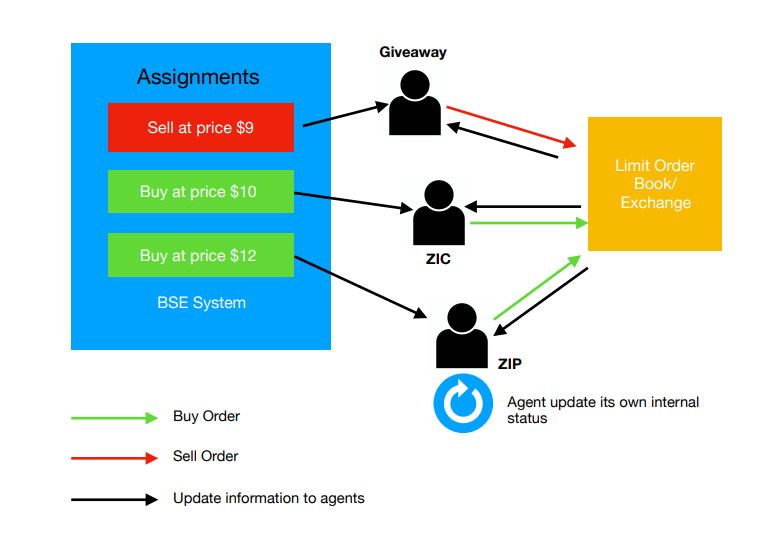
\includegraphics[ height=8cm]{BSE_figure}
\caption{McG's market model diagram} 
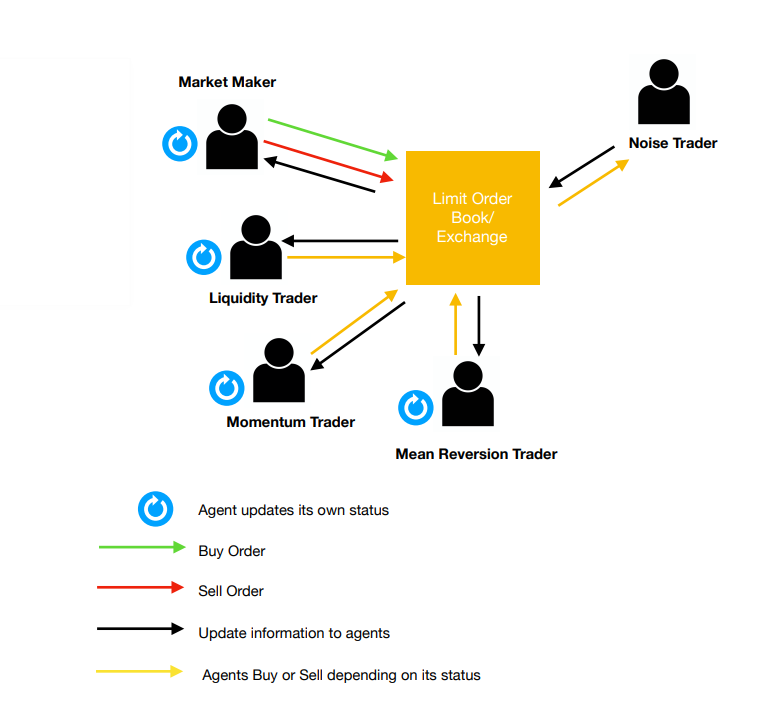
\includegraphics[width=\textwidth, height=10cm]{McGroarty_figure}
\end{figure} 

In the new implementation which this project is trying to achieve is finding a way to integrate these two systems so that the McG agents will be able to mimic the real market environment for the agents such as ZIP, ZIC and AA implemented in the BSE. This implementation requires a few changes.

\begin{itemize}
    \item  \textbf{Quantity} : The current version of the BSE does not support orders with quantity more than 1.This has to be change because all of McGroarty et al. agents require their market to be able to receive orders with quantity more than 1. 
    \item  \textbf{Accepting more than one order per round}: In the current version, the BSE only accepts one order randomly from an agent in a time step. Agents such as the Market maker must be able to submit more than one order in every round. 
    \item \textbf{Deleting an order} : The current version of the BSE does not fully support an agent cancelling their order directly. This has to be implemented as a part of the system since McGroarty et al. agents are capable of cancelling an order.
\end{itemize} 

\subsection{The availability of Best Price in the BSE}
Some of McG's agents depend on the "best price" of a side of the book in order to submit an order. However, unlike the real exchange market, the BSE does not always provide that, more specifically in the beginning of the trading day. This means that there must be some unavoidable modifications to the McG's agents condition regarding order submission. There are multiple approaches in which the project will explore, including:

\begin{itemize}
    \item \textbf{Not submitting if only the worst price is available} This simple makes sense because if the agent submits at the worst price, it is essentially making a loss, thus not a smart decision in any case. By skipping the round and waiting for the right market price is what any normal trader would do. 
    
    \item \textbf{Using the worst price with linear modification} * I'm not sure how to do this one yet so I'll be writing this one later 
\end{itemize} 

\bibliographystyle{plain} % We choose the "plain" reference style
\bibliography{research} % Entries are in the "refs.bib" file

\end{document}
